\documentclass{hw}
\usepackage{xcolor}
\usepackage{enumitem}

% STUDENTS: Please fill these out with your information
\newcommand{\name}{Matthew Shen}
\newcommand{\netid}{mds377}
\newcommand{\collaborators}{Hau Chu(hc793)}
% / STUDENT

\newcommand{\hwnum}{2}
\newcommand{\duedate}{October 17, 11:59pm ET}
\renewcommand{\title}{Dynamic programming and randomized algorithms}
\newcommand{\io}{\textbf{Code input and output format.} }

\newcommand{\submission}{\textbf{Submission.}}

\newtheorem{claim}{Claim}

\begin{document}

%%%%%%%%%%%%%%%%%%%%%%%%%%%%%%%%%%%%%%%%%%%%%%%%%%%%%%%%%%%%%%%%%%%%%%%%%%%%%%%%
% Problem 1: Non-adjacent sum

\begin{problem}
In this problem, you will compute the maximum sum of non-adjacent elements,
maxsum($x$), in two settings:
a list and a tree.
The definition of adjacent will be specific to each setting.
Additionally, for each setting you must first write out the subproblem
and then implement the full dynamic programming algorithm.

\begin{subproblem}
Given a sequence of integers $ x = x_1,x_2,\ldots,x_n $,
your goal is to compute the largest sum of non-adjacent elements of $x$,
maxsum\_list($x$).
Adjacent elements of the sequences are next to each other: $x_i$ and $x_{i+1}$.

(\textit{2 points}) Identify the dynamic programming subproblem and write its solution here.

(\textit{8 points}) Implement maxsum\_list in \texttt{problem\_1/p1\_a.py}.
\end{subproblem}

\io The input is a python list, and the output should be an integer.
Example: $\text{maxsum\_list}([2,1,3,4]) = 6$.

\begin{solution}
The following problem is a memoization problem. This is because we are looking at previously calculated max sum lists and determining if they can be improved upon as we go through the input list. We can think of the maximum sum of non-adjacent values in terms of looping through the entire list. As we go through the list the maximum sum of non-adjacent value is either the sum of our pointer and the previously calculated maximum sum of non-adjacent values or the value directly before our pointer. 

To start off we need to set up a series of edge cases. This includes when an empty list is given, a list with a single value is given, and a list with only two values is given. In these scenarios we return 0, the single value, and the maximum of the two values respectively. Next, we loop through the list and at each index we loop at which is larger, the previously stored value or the current value plus the value stored two indexes ago.

Once we fully loop through the list we can then return the last value.


\end{solution}

\begin{subproblem}
Given a tree with nodes that contain integers,
your goal is to compute the largest sum of non-adjacent elements.
Trees are represented as a set of vertices
$v_i \in V$ and edges $(v_i, v_j) \in E \subseteq V\times V$.
There are no loops and every vertex has at most a single parent.
Adjacent elements of the tree are those that have an edge between nodes, i.e. $(v_i,v_j)\in E$.
For convenience, define the children of a node to be $c(v_i) = \{v_j | (v_i,v_j)\in E\}$.

(\textit{2 points}) Identify the dynamic programming subproblem and write its solution here.

(\textit{8 points}) Implement the algorithm in \texttt{problem\_1/p1\_b.py}.
\end{subproblem}

\io The input is a tree represented as an adjacency list.
The adjacency list is a pair of dictions:
the first dictionary maps node names to node values,
and the second dictionary maps each vertex to a list of
child vertices.
The output should be an integer.
Example: $\text{maxsum\_tree}(\text{values} = \{2: 2, 1:1, 3:3, 4:4\}, \text{adjacency}=\{2: [1], 1: [3], 3: [4]\}) = 6$.


\end{problem}

\begin{solution}
For this problem memorization was also used. First the algorithm finds the root of the tree by looking for the node that is not a child of any other node. Next, a list is initialized that contains tuples. Each tuple has a node and whether or not the parent of that node is selected to be the max sum.

We start at the root node and first determine if the part node is selected. If the parent node is selected we then recursively calculate the max sum for if the node is part of the max sum and if the node is not part of the max sum. The larger of the two values is then selected. If the parent is already part of the max sum then we just need to calculate the max sum for all the children of that node. 

This information is then stored in the previously initialized list.
\end{solution}

\newpage

%%%%%%%%%%%%%%%%%%%%%%%%%%%%%%%%%%%%%%%%%%%%%%%%%%%%%%%%%%%%%%%%%%%%%%%%%%%%%%%%
% Problem 2

\newcommand{\rank}{\textnormal{rank}}
\newcommand{\Colon}{:}
\newcommand{\dotdot}{..}
\newcommand{\numinv}{\textrm{NI}}
\newcommand{\numlargeinv}{\textrm{NLI}}

\begin{problem}
  Given $n$ points in a 2D plane, your goal is to find the two points that are closest together
  according to the Euclidean distance $d(x,y) = \sum_i (x_i - y_i)^2$.

  \begin{subproblem}
    (\textit{5 points}) Implement a $O(n^2)$ brute-force method in \texttt{problem\_2/p2\_a.py}.
  \end{subproblem}

  \begin{subproblem}
    (\textit{5 points}) Implement the $O(n \log n)$ divide-and-conquer approach,
    described in Section 5.4 of Kleinberg and Tardos and the 9/12 lecture in \texttt{problem\_2/p2\_b.py}.
  \end{subproblem}

  \begin{subproblem}
    (\textit{10 points}) Implement the $O(n)$ randomized approach,
    described in Section 13.7 of Kleinberg and Tardos in \texttt{problem\_2/p2\_c.py}.
  \end{subproblem}

  \begin{subproblem}
      (\textit{5 points})
      Perform an empirical analysis of the three approaches,
      plotting their runtime performance for a series of problem sizes.
  \end{subproblem}

  \io The input is a list of tuples of floats corresponding to points in the plane.
  The output is a list of the two closest points.
  Ex2mple: $\text{closest\_points}([(0,0), (1,1), (5,5)]) = [(0,0), (1,1)]$
\end{problem}

\begin{solution}
For the empirical performance analysis the environment was:
        \begin{itemize}
            \item CPU: Intel(R) Core(TM) i7-8500Y CPU @ 1.50GHz (4 threads, 4.20GHz)
            \item OS \& Version: Debian GNU/Linux 11 (bullseye)
            \item Memory: 15.53 GB
        \end{itemize}
            
        The graph from the empirical performance analysis can be seen below:
\begin{figure}[ht]
  \centering
      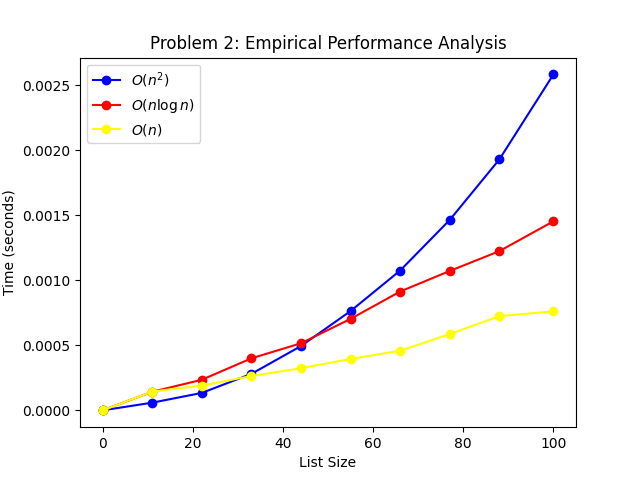
\includegraphics[width=0.5\textwidth]{figures/problem-2.png}
\end{figure}
From the graph we can see that initially the brute force method is the fastest; however, over time the the randomized algorithm and the divide and conquer algorithm becomes much faster.
\end{solution}
\newpage

%%%%%%%%%%%%%%%%%%%%%%%%%%%%%%%%%%%%%%%%%%%%%%%%%%%%%%%%%%%%%%%%%%%%%%%%%%%%%%%%
% Problem 3
\begin{problem}
\href{https://en.wikipedia.org/wiki/Skip_list}{Skip lists}
are randomized datastructures that allow efficient (in expectation)
insertion, search, and deletion operations in a sorted list.
We assume that list elements are always ints.

You will implement skip lists in this problem, as well as a linked list baseline.
We supply separate Node classes in each file \texttt{problem\_3/*.py}, which will be the backbone of each implementation.
Both implementions will have the following interface:
\begin{itemize}
\item insert(list, x: int) $\rightarrow$ None: Add a new int to our list.
\item search(list, x: int) $\rightarrow$ Node: Return the node in our list that has the value $x$.
\item delete(list, x: int) $\rightarrow$ None: the node in our list that has have value $x$.
\end{itemize}
For simplicity, we assume that no repeated elements will be inserted into the list.

Please read the following
\href{https://ocw.mit.edu/courses/6-046j-introduction-to-algorithms-sma-5503-fall-2005/resources/l12_skiplists/}{resource}
on skip lists for more helpful information.

\begin{subproblem}
(\textit{5 points}) As a baseline, implement a linked list class.
Give the runtime complexity of search, insertion, and deletion.
The linked list must always be in sorted order and all elements will be ints.
Include your implementation in \texttt{problem\_3/p3\_a.py}.
\end{subproblem}
\begin{solution}
For a linked list class searching for a variable will have a time complexity of $O(n)$. This is because you need to look through every variable in the list to find the one you are looking for. The time complexity of insertion is also $O(n)$. This is because at worst you are inserting the final value and have already looped through the entire linked list. Finally, the time complexity of deleting a value is $O(n)$. This is because in the worst case you are deleting the last value and you will have searched through the entire list.
\end{solution}


\begin{subproblem}
(\textit{5 points}) Implement insertion for skip lists, which should take $O(\log n)$ expected time.
All list elements will be ints.
Perform an empirical analysis of insertion in skip lists versus the linked list baseline.
Include your implementation in \texttt{problem\_3/p3\_b.py}.
\end{subproblem}
\begin{solution}
For the empirical performance analysis the environment was:
        \begin{itemize}
            \item CPU: Intel(R) Core(TM) i7-8500Y CPU @ 1.50GHz (4 threads, 4.20GHz)
            \item OS \& Version: Debian GNU/Linux 11 (bullseye)
            \item Memory: 15.53 GB
        \end{itemize}
            
        The graph from the empirical performance analysis can be seen below:
\begin{figure}[ht]
  \centering
      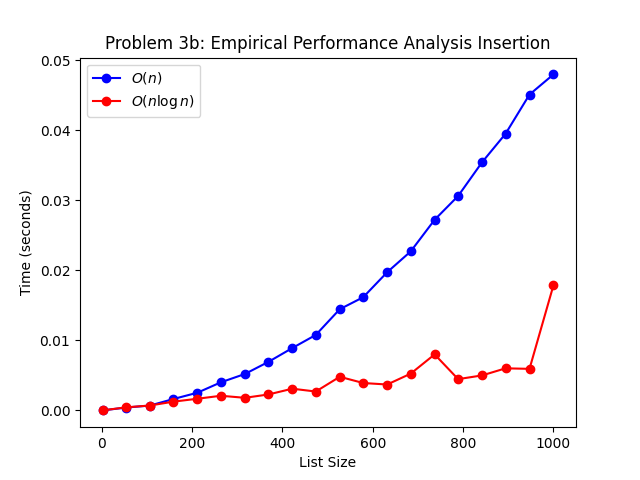
\includegraphics[width=0.5\textwidth]{figures/problem-3b.png}
\end{figure}

In the figure above we see that at the beginning the $O(n)$ algorithm runs faster; however, as the size of the list increases the $O(nlogn)$ is much faster. From a time complexity standpoint this does not make sense because $O(n)$ should be faster, but with the skip list, the majority of the time the algorithm is able to insert a value in less than $O(n)$. This means that in the later runs with bigger data sets, the $O(nlogn)$ is faster on average because it is unlikely it will face its worst case scenario.
\end{solution}


\begin{subproblem}
(\textit{5 points}) Implement search for skip lists, which should take $O(\log n)$ expected time.
Give the expected and worst-case runtime complexity.
All list elements will be ints.
Perform an empirical analysis of search in skip lists versus the linked list baseline.
Include your implementation in \texttt{problem\_3/p3\_b.py}.
\end{subproblem}
\begin{solution}
For the empirical performance analysis the environment was:
        \begin{itemize}
            \item CPU: Intel(R) Core(TM) i7-8500Y CPU @ 1.50GHz (4 threads, 4.20GHz)
            \item OS \& Version: Debian GNU/Linux 11 (bullseye)
            \item Memory: 15.53 GB
        \end{itemize}
            
        The graph from the empirical performance analysis can be seen below:
\begin{figure}[ht]
  \centering
      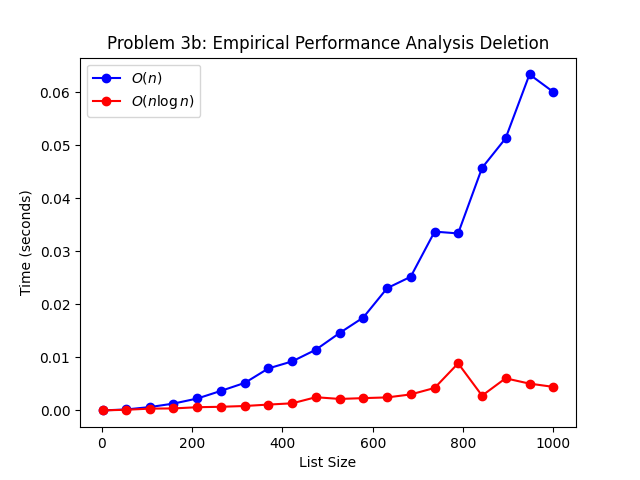
\includegraphics[width=0.5\textwidth]{figures/problem-3c.png}
\end{figure}

Similarly to part b, we see that at the beginning the $O(n)$ algorithm runs faster; however, as the size of the list increases the $O(nlogn)$ is much faster. As previously stated, the $O(n)$ algorithm is running at a slower speed than the $O(nlogn)$ because when the worst case scenario is not met, the average time needed to complete the $O(nlogn)$ algorithm is much faster.
\end{solution}


\begin{subproblem}
(\textit{5 points}) Implement deletion for skip lists, which should take $O(\log n)$ expected time.
All list elements will be ints.
Perform an empirical analysis of deletion in skip lists versus the linked list baseline.
Include your implementation in \texttt{problem\_3/p3\_b.py}.
\end{subproblem}
\begin{solution}
For the empirical performance analysis the environment was:
        \begin{itemize}
            \item CPU: Intel(R) Core(TM) i7-8500Y CPU @ 1.50GHz (4 threads, 4.20GHz)
            \item OS \& Version: Debian GNU/Linux 11 (bullseye)
            \item Memory: 15.53 GB
        \end{itemize}
            
        The graph from the empirical performance analysis can be seen below:
\begin{figure}[ht]
  \centering
      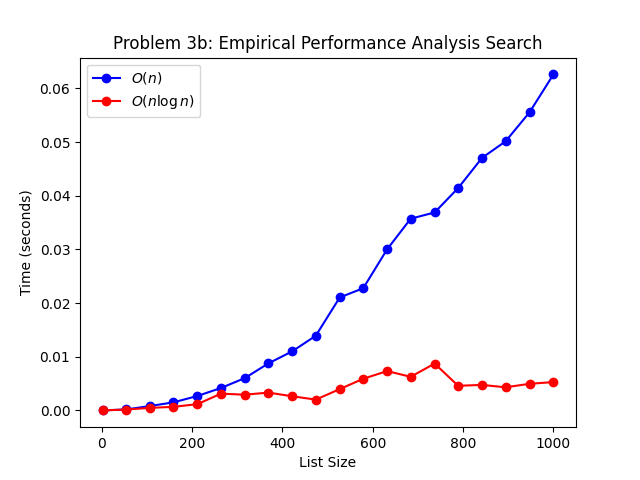
\includegraphics[width=0.5\textwidth]{figures/problem-3d.png}
\end{figure}

Similarly to part b and c, we see that at the beginning the $O(n)$ algorithm runs faster; however, as the size of the list increases the $O(nlogn)$ is much faster. Once again, this is an example of how the average run time is much faster for the $O(nlogn)$ while the worst case run time is faster for the $O(n)$ algorithm.
\end{solution}


Note: A deterministic alternative to skip lists are binary trees.
However, in order for binary trees to remain performant,
they must be balanced. Balanced binary tree implementations such as
AVL and Red-Black trees have relatively complicated implementations compared to skip lists.

\end{problem}
\newpage

%%%%%%%%%%%%%%%%%%%%%%%%%%%%%%%%%%%%%%%%%%%%%%%%%%%%%%%%%%%%%%%%%%%%%%%%%%%%%%%%
% Challenge 1
 
\begin{challenge}
    \textbf{\href{https://en.wikipedia.org/wiki/Partition_problem}{The number partition problem (NPP)}}

    Given a multi-set of $n$ integers $S$,
    our goal is to find a partitioning of this set into $A\subset S$ and $B\subset S$
    in order to minimize their difference $|\sum_{a\in A}a - \sum_{b\in B}b|$.
    Please include all of your implementations in \texttt{challenge\_1/partition.py}.

    \begin{enumerate}[label={(\alph*)}]
        \item (\textit{5 points}) Implement a brute-force approach that operates in exponential time.

        \item (\textit{5 points}) Describe and implement a greedy approximation algorithm for this problem.
        
        \begin{solution}
        Please answer here.
        \end{solution}

        \item (\textit{5 points}) Describe and implement an exact dynamic programming approach.

        \begin{solution}
        Please answer here.
        \end{solution}

        \item(\textit{5 points}) Perform an empirical analysis of the approaches, reporting their runtime for different problem sizes as well as their accuracy for problem sizes where exact solutions are feasible.
    
        \begin{solution}
        Please answer here.
        \end{solution}

    \end{enumerate}


    \io The input $x=x_1 \ldots x_n$ is a list of $n$ integers.
    The output should be a vector of 0's and 1's
    indicating the partitioning of the input into $A$ and $B$.
    The first element of the output should always be 0, indicating membership $x_1 \in A$.
\end{challenge}

%%%%%%%%%%%%%%%%%%%%%%%%%%%%%%%%%%%%%%%%%%%%%%%%%%%%%%%%%%%%%%%%%%%%%%%%%%%%%%%%
% Challenge 2

\begin{challenge}
    In this challenge problem we will solve the {\em sequence alignment problem}. The approach we will implement is discussed in detail in Kleinberg and Tardos Sections 6.6 and 6.7.
    
    In the sequence alignment problem, we are given two sequences $x=x_1\ldots x_n$ and
    $y=y_1\ldots y_m$, as well as a cost function $c(x_i,y_j)$ that measures element-wise similarity.
    We denote $\delta$ as the cost for not aligning an element to anything,
    or aligning an element to a gap.
    The goal is to match up or align elements of $x$ to elements of $y$ that are similar.
    This is formalized as a minimum cost alignment between $x$ and $y$,
    where a lower total cost implies that $x$ and $y$ are similar.
    
    Formally, an alignment $A$ is a set of ordered pairs that denote which elements $x_i \in x$ are matched with elements $y_j \in y$.
    Alignments have two properties:
    each element in $x$ and $y$ is aligned to at most one other element in the other sequence
    and there are no crossing pairs: if $(i, j), (i', j') \in A$ and $i < i'$, then $j < j'$.
    The cost of an alignment is the cost of each of the aligned elements. 
    
    For example,
    \begin{verbatim}
        stop-
        -tops
    \end{verbatim}
    corresponds to the alignment $[(2,1), (3,2), (4,3)]$ and has cost
    $$\delta + c(t,t) + c(o,o) + c(p,p) + \delta.$$
    Elements aligned to gaps - are not included in the final list-of-tuples representation of the alignment.
    
    \begin{enumerate}[label={(\alph*)}]
    \item (\textit{5 points})
    Implement the $O(nm)$ dynamic programming algorithm described on page 282 of Kleinberg and Tardos in \texttt{challenge\_2/seq\_alignment\_a.py}.
    This algorithm is known as the \href{https://en.wikipedia.org/wiki/Needleman-Wunsch\_algorithm}{Needleman-Wunsch algorithm}.
    
    
    \item(\textit{15 points})
    The above approach utilized $O(nm)$ space.
    Utilize a divide-and-conquer approach to reduce the space to $O(n+m)$
    while keeping the running time complexity of $O(nm)$,
    following section 6.7 of Kleinberg and Tardos.
    This algorithm is known as \href{https://en.wikipedia.org/wiki/Hirschberg's\_algorithm}{Hirschberg's algorithm}.
    Include your implementation in \texttt{ challenge\_2/seq\_alignment\_b.py}.
    \end{enumerate}

    
    \io The input is two strings, the cost function $c$, and gap penalty $\delta$
    align($x$, $y$, $c$, $\delta$).
    For example, $x = $ "abcd", $y=$ "bcde",
    \begin{verbatim}
    def c(a, b):
        return 0 if a == b else 1
    \end{verbatim}
    and $\delta = 1$.
    The output should be the list of tuples corresponding to the alignment and the cost of the alignment:
    $[(2,1), (3,2), (4,3)]$ and cost 2.
    
    
    While sequence alignment of two sequences is relatively solved,
    the problem of aligning multiple sequences is not.
    This is referred to as multiple sequence alignment (MSA),
    and is under \href{https://academic.oup.com/bioinformatics/article/39/1/btac724/6820925}{active research}.
\end{challenge}

\begin{solution}
No written component for this problem :)
\end{solution}


\end{document}
